\documentclass{ximera}

\newcommand{\dfn}{\textbf}
\renewcommand{\vec}[1]{{\overset{\boldsymbol{\rightharpoonup}}{\mathbf{#1}}}\hspace{0in}}
%% Simple horiz vectors
\renewcommand{\vector}[1]{\left\langle #1\right\rangle}
\newcommand{\arrowvec}[1]{{\overset{\rightharpoonup}{#1}}}
\newcommand{\R}{\mathbb{R}}
\newcommand{\transpose}{\intercal}
\newcommand{\ro}{\texttt{R}}%% row operation
\newcommand{\dotp}{\bullet}%% dot product

\usetikzlibrary{calc,bending}
\tikzset{>=stealth}


\usepackage{mdframed} % For framing content
%\usepackage{ifthen}   % For conditional statements

% Define the 'concept' environment with an optional header
\newenvironment{concept}[1][]{%
  \begin{mdframed}[linecolor=black, linewidth=2pt, innertopmargin=5pt, innerbottommargin=5pt, skipabove=12pt, skipbelow=12pt]%
    \noindent\large\textbf{#1}\normalsize%
}{%
  \end{mdframed}%
}











%% \colorlet{textColor}{black}
%% \colorlet{background}{white}
%% \colorlet{penColor}{blue!50!black} % Color of a curve in a plot
%% \colorlet{penColor2}{red!50!black}% Color of a curve in a plot
%% \colorlet{penColor3}{red!50!blue} % Color of a curve in a plot
%% \colorlet{penColor4}{green!50!black} % Color of a curve in a plot
%% \colorlet{penColor5}{orange!80!black} % Color of a curve in a plot
%% \colorlet{penColor6}{yellow!70!black} % Color of a curve in a plot
%% \colorlet{fill1}{penColor!20} % Color of fill in a plot
%% \colorlet{fill2}{penColor2!20} % Color of fill in a plot
%% \colorlet{fillp}{fill1} % Color of positive area
%% \colorlet{filln}{penColor2!20} % Color of negative area
%% \colorlet{fill3}{penColor3!20} % Fill
%% \colorlet{fill4}{penColor4!20} % Fill
%% \colorlet{fill5}{penColor5!20} % Fill
%% \colorlet{gridColor}{gray!50} % Color of grid in a plot


\author{Parisa Fatheddin and Bart Snapp}

\title{Matrices, products, and \textcolor{blue}{systems of} equations}


\begin{document}
\begin{abstract}
  A concrete introduction to \textcolor{blue}{take out vectors and}\underline{vectors and} matrices, with an informal
  view towards vector spaces and linear transformations.
\end{abstract}
\maketitle



A \dfn{matrix} is just a large rectangular array of numbers
\[
M =
\underset{\displaystyle\boldsymbol{5}~\textbf{columns}}{\begin{pmatrix}
  a_{1,1} & a_{1,2} & a_{1,3} & a_{1,4} & a_{1,5} \\
  a_{2,1} & a_{2,2} & a_{2,3} & a_{2,4} & a_{2,5} \\
  a_{3,1} & a_{3,2} & a_{3,3} & a_{1,4} & a_{3,5} \\
  a_{4,1} & a_{4,2} & a_{4,3} & a_{4,4} & a_{4,5}
\end{pmatrix}}
\boldsymbol{4}~\textbf {rows}
\]
We give the \dfn{dimensions of a matrix} by stating its number of rows
and columns. The number of rows comes first and the number of columns second, so $M$ above is
a $(4\times 5)$-matrix. We can use similar notation to talk about
specific entries of a matrix. Above, $a_{i,j}$ is the
$\boldsymbol{(i,j)}${\bf-}\dfn{entry} of the matrix $M$. Sometimes people write $M_{i,j}$ to mean the $(i,j)$-entry of the matrix $M$.

\begin{question}
  a. Which of the following matrices are $3\times 2$ matrices?
  \begin{multipleChoice}
  \choice{\[\left(\begin{array}{ccc}
  2 & 4 & 8\\
  5 & 9 & -1\\
  6 & 0 & 1
  \end{array}\right)\]}
  \choice{\[\left(\begin{array}{ccc}
  0 & 1 &3\\
  0 & 0 & 2
  \end{array}\right)\]}
  \choice[correct]{\[\left(\begin{array}{cc}
  2 & 1 \\
  4 & 5 \\
  -1 & 0
  \end{array}\right)\]}
  \choice[correct]{\[\left(\begin{array}{cc}
  1 & -1\\
  -3 & 0 \\
  0 & 0
  \end{array}\right)\]}
  \choice{\[ \left(\begin{array}{ccc}
  0 & 0 & 0\\
  -1 & 0 & 5
  \end{array}\right)\]}
\end{multipleChoice}
  b. If
  \[A= \left(\begin{array}{ccc}
  -3 & 0 & 1\\
  4 & 5 & -2\\
  0 & 9 & -1
  \end{array}\right)\]
  what are the entries $a_{12},\hspace{.08cm} a_{22}, \hspace{.08cm}a_{32}$?
  \begin{prompt}
  \begin{equation*}
  a_{12} = \answer[given]{0}, \hspace{.5cm} a_{22} = \answer[given]{5}, \hspace{.5cm} a_{32} = \answer[given]{9}
  \end{equation*}
  \end{prompt}
\end{question}
In fact $n$-dimensional row vectors are just $1\times n$ matrices and
$n$-dimensional column vectors are just $n\times 1$ matrices\textcolor{blue}{:
\[
\left(\begin{array}{cccc} a_{1} & a_{2} & \cdot \cdot \cdot & a_{n}\end{array}\right), \hspace{.5cm} \begin{pmatrix} a_{1}\\
a_{2}\\
\cdot\\
\cdot\\
\cdot\\
a_{n}\end{pmatrix}
\]}


\section{Matrices store data}


\textcolor{blue}{A matrix} \underline{Matrices} can be thought of as a ``mathematical spreadsheet.'' With a
spreadsheet you have rows and columns of data.  You can think of a
matrix as vectors stacked together either horizontally
or vertically.

\begin{example}[Population Counts] %https://worldpopulationreview.com/states/states-by-race
  \textcolor{blue}{In an example in Chapter One,} \underline{In a previous example,} we encoded the $2023$
  \link[demographics]{https://worldpopulationreview.com/states/states-by-race}~of
  the twelve Midwestern States as $6$-dimensional vectors represented
  as ordered tuples. Represent this data by a $12\times 6$
  matrix. Explain what the entry at position $(7,5)$ represents.
  \begin{explanation}
  Since ordered-tuples are \wordChoice{\choice[correct]{horizontal}\choice{vertical}} it makes sense to
  concatenate this data by stacking it horizontally into a matrix:
  \[
  \begin{pmatrix}
  \vec{p}_{\texttt{IA}} \\
  \vec{p}_{\texttt{IL}} \\
  \vec{p}_{\texttt{IN}} \\
  \vec{p}_{\texttt{KA}} \\
  \vec{p}_{\texttt{MI}} \\
  \vec{p}_{\texttt{MN}} \\
  \vec{p}_{\texttt{MO}} \\
  \vec{p}_{\texttt{ND}} \\
  \vec{p}_{\texttt{NE}} \\
  \vec{p}_{\texttt{OH}} \\
  \vec{p}_{\texttt{SD}} \\
  \vec{p}_{\texttt{WI}}
  \end{pmatrix}
  =
  \begin{pmatrix}
  2806418 & 117035 & 10538 & 79296 & 3941 & 132783\\
  8874067 & 1796660 & 33972 & 709567 & 5196 & 1296702\\
  5510354 & 631923 & 14030 & 158705 & 2205 & 379676\\
  2416165 & 165837 & 22278 & 87093 & 2344 & 218902\\
  7735902 & 1360149 & 50035 & 316844 & 3117 & 507860\\
  4572149 & 359817 & 54558 & 275242 & 2201 & 336199\\
  4978046 & 698043 & 24274 & 123810 & 8887 & 291100\\
  651470 & 23959 & 39165 & 11979 & 1004 & 32817\\
  1641256 & 91896 & 16875 & 47944 & 1235 & 124620\\
  9394878 & 1442655 & 20442 & 268527 & 3907 & 544866\\
  735228 & 18836 & 74975 & 12413 & 544 & 37340\\
  4895065 & 367889 & 48674 & 163396 & 2672 & 329279
  \end{pmatrix}
  \]
  Note that the above is a $12\times 6$ matrix. The $(7, 5)$- entry is $8887$ which is the number of Hawaiians in Missouri (MO).
  \end{explanation}
\end{example}



\begin{example}[RGB Color Space]
  \textcolor{blue}{In an example in Chapter One,}In a previous example we mentioned an LED table lamp whose shades
  vary linearly through the RGB color space in this order:
  \begin{center}
    red, yellow, \textcolor{blue}{green}, cyan, blue, magenta
  \end{center}
  Represent this sequence of RGB colors by a $\textcolor{blue}{3 times 6}5\times 3$
  matrix. Interpret the meaning of the $(2,3)$-entry of the matrix.
  \begin{explanation}
    Let's start by finding the RGB colors \textcolor{blue}{(better to list all as in the example so they can have it)}:
    \[
    \underset{red}{\begin{pmatrix}255\\0\\0\end{pmatrix}}
    \]
    \textcolor{blue}{
    \[
    \underset{\text{red}}{\begin{pmatrix}255\\0\\0\end{pmatrix}},
    \underset{\text{yellow}}{\begin{pmatrix}255\\255\\0\end{pmatrix}},
    \underset{\text{green}}{\begin{pmatrix}0\\255\\0\end{pmatrix}},
    \underset{\text{cyan}}{\begin{pmatrix}0\\255\\255\end{pmatrix}},
    \underset{\text{blue}}{\begin{pmatrix}0\\0\\255\end{pmatrix}},
    \underset{\text{magenta}}{\begin{pmatrix}255\\0\\255\end{pmatrix}},
    \]
    Since we are using column vectors, we'll concatenate this data by
    placing the vectors side-by-side:
    \[
    \begin{pmatrix}
    255 & 255 & 0 & 0 & 0 & 255\\
    0 & 255& 255 & 255 & 0 & 0 \\
    0 & 0 & 0 & 255 & 255 & 255 
    \end{pmatix}
    \]
    The meaning of the $(2,3)$-entry is BADBAD 
  \end{explanation}
\end{example}





\section{Multiplying vectors and matrices}

Baby-steps to multiplying matrices! We'll start by multiplying a $(1\times 3)$-matrix by a $(3\times 1)$ matrix
\[
\begin{pmatrix} a_{1,1} & a_{1,2} & a_{1,3} \end{pmatrix}
\begin{pmatrix} b_{1,1} \\ b_{2,1} \\ b_{3,1} \end{pmatrix} = a_{1,1}b_{1,1} + a_{1,2}b_{2,1} + a_{1,3}b_{3,1}
\]
This is equivalent to multiplying a row vector by a column vector. We
can imagine a `physical' movement of the entries with this product:

\begin{center}
  \begin{tikzpicture}
    \draw[line width=18pt, black!20!white, ->] (-.95,-.4) -- (-.95, .8) -- (-3,.8 );
    \node at (0,0) {\begin{minipage}{\textwidth}
        \begin{align*}
          \begin{pmatrix} a_{1,1} & a_{1,2} & a_{1,3} \end{pmatrix}
          \begin{pmatrix} b_{1,1} \\ b_{2,1} \\ b_{3,1} \end{pmatrix} &=
          \begin{pmatrix} a_{1,1} & a_{1,2} & a_{1,3} \end{pmatrix}\begin{pmatrix} \phantom{b_{1,1}} \\ \phantom{b_{2,1}} \\ \phantom{b_{3,1}} \end{pmatrix}\\
          &= \substack{b_{1,1}\\ \cdot \\a_{1,1}} + \substack{b_{2,1}\\ \cdot \\a_{1,2}} + \substack{b_{3,1}\\\cdot \\ a_{1,3}}\\
          &= a_{1,1}b_{1,1} + a_{1,2}b_{2,1} + a_{1,3}b_{3,1}
        \end{align*}
      \end{minipage}};
    \node at (1.5,.7) {$\begin{matrix} b_{1,1} & b_{1,2} & b_{1,3} \end{matrix}$};
  \end{tikzpicture}
\end{center}
Note that this multiplication results in a scalar not a vector. We'll leave it to the reader to generalize the procedure to $(1\times n)$-matrix by a $(n\times 1)$ matrix.

\begin{question}
 Perform the following multiplication if possible (write N/A if it is not possible):
 \[
 \left(\begin{array}{cccc}
 4 & 1 & 2 & -1
 \end{array}\right)\left(\begin{array}{c}
 0\\
 5\\
 -2\\
 7
 \end{array}\right) = \answer[given]{0} + \answer[given]{5}+\answer[given]{-4} + \answer[given]{-7} = \answer[given]{-6}
 \]
\end{question}




This type of vector/matrix multiplication is so important, it has it's own name.

\begin{definition}
  The \dfn{dot product} or \dfn{scalar product} of two vectors
  $\vec{v}$ and $\vec{w}$ is given by:
  \[
  \vec{v}\dotp \vec{w} =  \vec{v}^\transpose \vec{w}.
  \]
\end{definition}

The first thing you should notice about the dot product is that
\[
\mathbf{vector}\dotp \mathbf{vector} = \mathbf{number}.
\]


\begin{question}
  Compute:
  \[
  \begin{pmatrix} 1 & 1 & -1 \end{pmatrix}
  \dotp\begin{pmatrix} 1 & 1 & 2\end{pmatrix}\]
  \begin{prompt}
     \[=\left(\begin{array}{ccc} \answer[given]{1} & \answer[given]{1} & \answer[given]{-1}\end{array}\right) \begin{pmatrix} 1\\
    \answer[given]{1}\\
    \answer[given]{1}\\
    \answer[given]{2}
    \end{pmatrix}= \answer[given]{0}
    \]
  \end{prompt}
\end{question}




\begin{warning}
  There is no general way to ``multiply'' vectors of the same type and
  have the resulting product be a reasonable vector also of that type.
  You might think it is reasonable to define
  \begin{center}
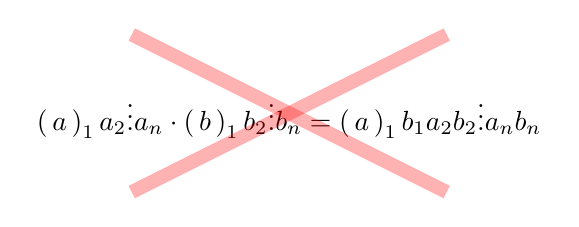
\begin{tikzpicture}
    \node at (0,0) {
      $\begin{pmatrix}
        a_1\\
        a_2\\
        \vdots\\
        a_n
      \end{pmatrix}
      \cdot
      \begin{pmatrix}
        b_1\\
        b_2\\
        \vdots\\
        b_n
      \end{pmatrix}
      =
      \begin{pmatrix}
        a_1b_1\\
        a_2b_2\\
        \vdots\\
        a_nb_n
      \end{pmatrix}$};
    \draw[red, line width=5pt,opacity=.3] (-2,-1) -- (2,1);
    \draw[red, line width=5pt,opacity=.3] (-2,1) -- (2,-1);
\end{tikzpicture}
  \end{center}
but this operation is not especially useful, and will \textbf{never be
  utilized in this course}.
\end{warning}

\begin{question}
  Let $\vec{u},\vec{v},\vec{w}$ be nonzero vectors of the same dimension. Which of
  the following expressions make sense?
  \begin{selectAll}
    \choice[correct]{$(\vec{w} \dotp \vec{u} ) \vec{u}$}
    \choice[correct]{$5(\vec{u} +\vec{w}) \dotp {\vec{u}}$}
    \choice{$\vec{w} / \vec{u}$}
    \choice[correct]{$(2,3) \dotp (4,2) + 7$}
    \choice[correct]{$\vec{w} / ( \vec{u} \dotp \vec{u})$}
    \choice{$(1,3) \dotp (-1,2,5)$}
    \choice{$\vec{u}\dotp \vec{v}+\vec{w}$}
  \end{selectAll}
  \begin{hint}
    Think about which terms/factors are vectors and which
    terms/factors are scalars.
  \end{hint}
  \begin{question}
    Which of the following are vectors?
    \begin{selectAll}
    \choice[correct]{$(\vec{w} \dotp \vec{u} ) \vec{u}$}
    \choice{$5(\vec{u} +\vec{w}) \dotp {\vec{u}}$}
    \choice{$(2,3) \dotp (4,2) + 7$}
    \choice[correct]{$\vec{w} / ( \vec{u} \dotp \vec{u})$}
    \end{selectAll}
  \end{question}




To multiply a matrix by a column vector, envision the matrix as a
grouping of row vectors and use the distributive property. For
example:
\begin{align*}
\begin{pmatrix}
  a_{1,1} & a_{1,2} & a_{1,3} \\
  a_{2,1} & a_{2,2} & a_{2,3} \\
  a_{3,1} & a_{3,2} & a_{3,3}
\end{pmatrix}
\begin{pmatrix} b_{1,1} \\ b_{2,1} \\ b_{3,1} \end{pmatrix}
&=
\begin{pmatrix}
  (a_{1,1} & a_{1,2} & a_{1,3}) \\
  (a_{2,1} & a_{2,2} & a_{2,3}) \\
  (a_{3,1} & a_{3,2} & a_{3,3})
\end{pmatrix}
\begin{pmatrix} b_{1,1} \\ b_{2,1} \\ b_{3,1} \end{pmatrix}\\
&=
\begin{pmatrix}
  (a_{1,1} & a_{1,2} & a_{1,3}) \begin{pmatrix} b_{1,1} \\ b_{2,1} \\ b_{3,1} \end{pmatrix}\\
  (a_{2,1} & a_{2,2} & a_{2,3}) \begin{pmatrix} b_{1,1} \\ b_{2,1} \\ b_{3,1} \end{pmatrix}\\
  (a_{3,1} & a_{3,2} & a_{3,3}) \begin{pmatrix} b_{1,1} \\ b_{2,1} \\ b_{3,1} \end{pmatrix}
\end{pmatrix}\\
&=
\begin{pmatrix}
  a_{1,1}b_{1,1} + a_{1,2}b_{2,1} + a_{1,3}b_{3,1}  \\
  a_{2,1}b_{1,1} + a_{2,2}b_{2,1} + a_{2,3}b_{3,1}  \\
  a_{3,1}b_{1,1} + a_{3,2}b_{2,1} + a_{3,3}b_{3,1}
\end{pmatrix}
\end{align*}

We're basically multiplying each shaded section below by the column vector

\begin{center}
  \begin{tikzpicture}
    \draw[red!30!white,line width = 1.3em] (-4.5,.45) -- (-2,.45);
    \draw[blue!20!white,line width = 1.3em] (-4.5,0) -- (-2,0);
    \draw[green!20!white,line width = 1.3em] (-4.5,-.45) -- (-2,-.45);

    \draw[red!30!white,line width = 1.3em] (.2,.45) -- (4.4,.45);
    \draw[blue!20!white,line width = 1.3em] (.2,0) -- (4.4,0);
    \draw[green!20!white,line width = 1.3em] (.2,-.45) -- (4.4,-.45);

    \node at (0,0)
          {$\begin{pmatrix}
              a_{1,1} & a_{1,2} & a_{1,3} \\
              a_{2,1} & a_{2,2} & a_{2,3} \\
              a_{3,1} & a_{3,2} & a_{3,3}
            \end{pmatrix}
            \begin{pmatrix} b_{1,1} \\ b_{2,1} \\ b_{3,1} \end{pmatrix}
            =
            \begin{pmatrix}
              a_{1,1}b_{1,1} + a_{1,2}b_{2,1} + a_{1,3}b_{3,1}  \\
              a_{2,1}b_{1,1} + a_{2,2}b_{2,1} + a_{2,3}b_{3,1}  \\
              a_{3,1}b_{1,1} + a_{3,2}b_{2,1} + a_{3,3}b_{3,1}
            \end{pmatrix}$};
  \end{tikzpicture}
\end{center}





\begin{warning}
  It only makes sense to multiply a matrix by a column vector if the
  number of columns of the matrix equals the dimension of the column
  vector.
\end{warning}
As a general rule, we can multiply matrix, $A: n \times m$ by matrix $B: k \times \ell$ if $m=k$. That is if the middle two numbers match: $n\times \underline{m} \hspace{.5cm} \underline{k} \times \ell$. The result then turns out to be a matrix of size $n\times \ell$ (the outside numbers).

In an entirely similar way, we can multiply a row vector by a matrix
by envisioning the matrix as a grouping of column vectors. In this
case, we will use a $2$-dimensional row vector and a $2\times2$ matrix
to save horizontal space.

\begin{align*}
\begin{pmatrix} a_{1,1} & a_{1,2}  \end{pmatrix}
\begin{pmatrix}
  b_{1,1} & b_{1,2} \\
  b_{2,1} & b_{2,2}
\end{pmatrix}
&=
\begin{pmatrix} a_{1,1} & a_{1,2}  \end{pmatrix}%\arraycolsep=0pt
\begin{pmatrix}
  \begin{pmatrix} b_{1,1} \\ b_{2,1} \\  \end{pmatrix} &
  \begin{pmatrix} b_{1,2} \\ b_{2,2} \\ \end{pmatrix}
\end{pmatrix} \\
&=
\begin{pmatrix}
  \begin{pmatrix} a_{1,1} & a_{1,2} \end{pmatrix}\begin{pmatrix} b_{1,1} \\ b_{2,1} \end{pmatrix} &
  \begin{pmatrix} a_{1,1} & a_{1,2} \end{pmatrix}\begin{pmatrix} b_{1,2} \\ b_{2,2} \end{pmatrix}
\end{pmatrix}\\
&=
\begin{pmatrix}
a_{1,1}b_{1,1}+a_{1,2}b_{2,1} &
a_{1,1}b_{1,2}+a_{1,2}b_{2,2}
\end{pmatrix}
\end{align*}


%% \begin{align*}
%% &\begin{pmatrix} a_{1,1} & a_{1,2} & a_{1,3} \end{pmatrix}
%% \begin{pmatrix}
%%   b_{1,1} & b_{1,2} & b_{1,3} \\
%%   b_{2,1} & b_{2,2} & b_{2,3} \\
%%   b_{3,1} & b_{3,2} & b_{3,3}
%% \end{pmatrix}
%% =
%% \begin{pmatrix} a_{1,1} & a_{1,2} & a_{1,3} \end{pmatrix}\arraycolsep=0pt
%% \begin{pmatrix}
%%   \begin{pmatrix} b_{1,1} \\ b_{2,1} \\ b_{3,1} \end{pmatrix} &
%%   \begin{pmatrix} b_{1,2} \\ b_{2,2} \\ b_{3,2} \end{pmatrix} &
%%   \begin{pmatrix} b_{1,3} \\ b_{2,3} \\ b_{3,3} \end{pmatrix}
%% \end{pmatrix} \\
%% &=\arraycolsep=0pt
%% \begin{pmatrix}
%%   \begin{pmatrix} a_{1,1} & a_{1,2} & a_{1,3} \end{pmatrix}\begin{pmatrix} b_{1,1} \\ b_{2,1} \\ b_{3,1} \end{pmatrix} &
%%   \begin{pmatrix} a_{1,1} & a_{1,2} & a_{1,3} \end{pmatrix}\begin{pmatrix} b_{1,2} \\ b_{2,2} \\ b_{3,2} \end{pmatrix} &
%%   \begin{pmatrix} a_{1,1} & a_{1,2} & a_{1,3} \end{pmatrix}\begin{pmatrix} b_{1,3} \\ b_{2,3} \\ b_{3,3} \end{pmatrix}
%% \end{pmatrix}\\
%% &=\arraycolsep=0pt
%% \begin{pmatrix}
%% a_{1,1}b_{1,1}+a_{1,2}b_{2,1}+a_{1,3}b_{3,1} &
%% a_{1,1}b_{1,2}+a_{1,2}b_{2,2}+a_{1,3}b_{3,2} &
%% a_{1,1}b_{1,3}+a_{1,2}b_{2,3}+a_{1,3}b_{3,3}
%% \end{pmatrix}
%% \end{align*}



\begin{warning}
  It only makes sense to multiply a row vector by a matrix if the
  dimension of the row vector equals the number of rows of the
  matrix.
\end{warning}

\begin{example}[Population Counts]
Extract a new data set from a matrix using basis vectors
\end{example}


\begin{example}[RGB Color Space]
\end{example}



\section{Matrices transform data}


\begin{example}[Financial Transactions]
  Recall that a bookstore sells a variety of books with each type of
  book sold in one month stored as a row vector
  \[
  \vec{s} = \begin{pmatrix}141 & 304 & 249 & 199 & 251 \end{pmatrix}
  \]
  with the entries representing the categories: Science Fiction,
  Fantasy, Mystery, Romance, Historical in that order.  Suppose last
  month the book store bought $200$ Science Fiction, $400$ Fantasy, $300$
  Mystery, $250$ Romance, $300$ Historical books. What percentage of each
  category was sold this month?
  \begin{explanation}
    Let
    \[
    T =
    \begin{pmatrix}
      100/200 & 0 &    0   &   0    &   0 \\
      0 & 100/400 &    0   &   0    &   0 \\
      0 &   0   &  100/300 &   0    &   0 \\
      0 &   0   &    0   & 100/250  &   0 \\
      0 &   0   &    0   &   0    & 100/300
    \end{pmatrix}
    \]
    Each entry of the matrix $T$ is of the form:
    \[
    100 \cdot \frac{1}{(\text{Stock})}
    \]
    where $(\text{Stock})$ represents the number of books the
    bookstore bought to sell.  We can solve our problem by computing
    \[
    \vec{s} T =
    \]
    So we see
  \end{explanation}

\end{example}




\begin{example}[Navigation]
  Scale/normalize fincinal data etc.
\end{example}



For some interesting extra reading check out:
\begin{itemize}
\item \link[\textit{Earliest Uses of Symbols for Matrices and Vectors},  MacTutor History of Mathematics, (University of St Andrews, Scotland, February 2000.]{https://mathshistory.st-andrews.ac.uk/Miller/mathsym/matrices/}
\end{itemize}



\end{document}
